The ECAL measures both the energy deposited in the calorimeter by incident particles, and the time at which that energy was deposited. In both cases these measurements are extrapolated from the scintillating light pulse produced when the incident particle interacts with the PbWO$_{4}$ crystal.  When a particle is incident in a PbWO$_{4}$ crystal, it will produce an electromagnetic shower of electron - positron pairs and photons. The showering particles will dissipate their energy through ionization, leading to the excitation of the scintillating centers of the PbWO$_{4}$ crystal. The scintillating centers will de-excite producing a pulse of scintillating light at a specific wavelength that is proportional to the energy of the original, incident particle. The "signal" pulse is amplified and shaped by the readout electronics, thereby defining the shape of the pulse \cite{Karimäki:368412}. This shape is constant for all sampled pulses in a particular crystal ( or channel ) and is very well known. Ten consecutive amplitude samples of this "signal" pulse are recorded. In Figure~\ref{tec_pulseshape} the time structure of a typical signal pulse shape as measured after amplification (solid line) is shown. The normalized amplitude of the pulse, $A/A_{max}$, is a function of the time difference T-T$_{max}$, where T$_{max}$ is defined as the time when the pulse reaches its maximum value. The dots are the ten discrete samples of the pulse amplitude.
%, as typical in a single event, with the pedestal amplitude subtracted and normalized to the maximum amplitude. 

\begin{figure}[htbp]
\begin{center}
\resizebox{0.75\linewidth}{!}{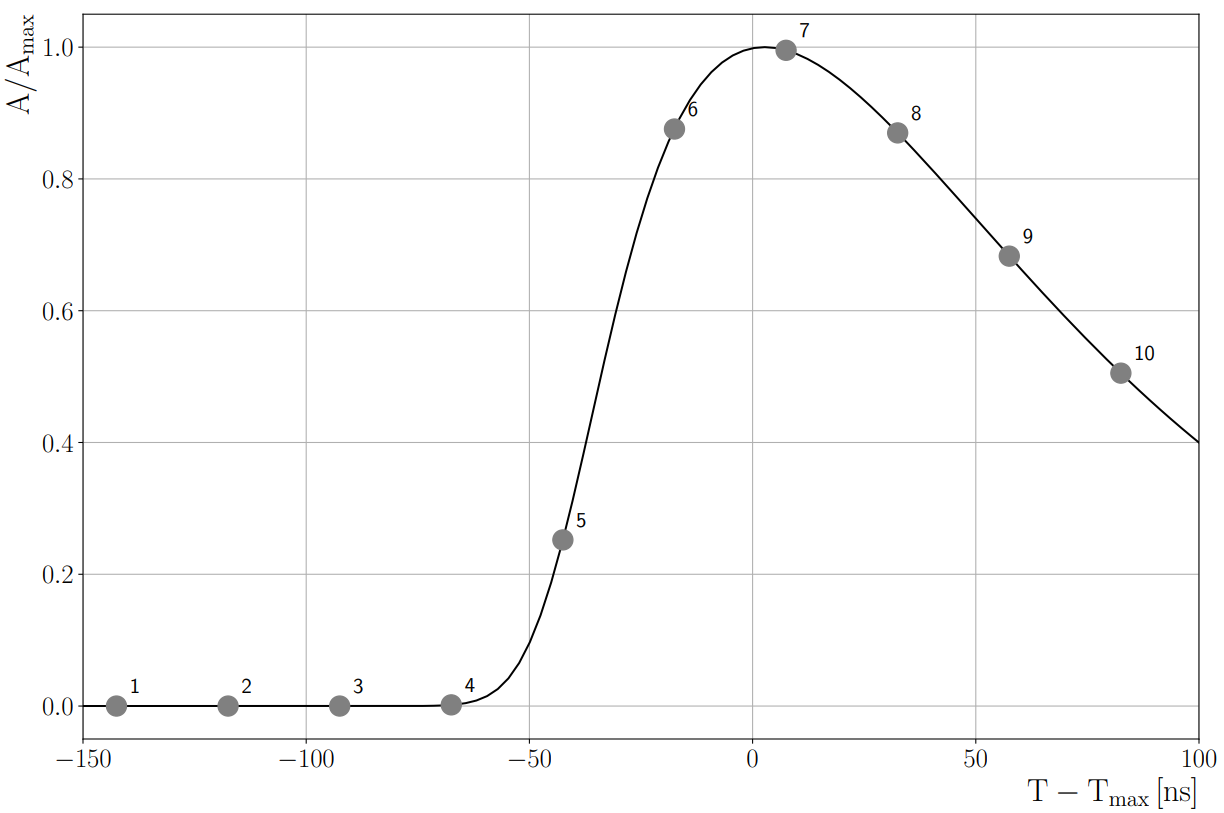
\includegraphics{fig/sec_reco/pulse_template.png}}
\caption{The typical pulse shape measured in the ECAL, as a function of the difference between the time (T) of the ADC sample and the time (Tmax) of the maximum of the pulse and the amplitude of the pulse (A) normalized by the maximum amplitude of the pulse (A$_{max}$).  The dots indicate ten discrete samples of the pulse as taken from a single event with the pedestal ( the amplitude measured when no pulse is present ) subtracted.}
\label{tec_pulseshape}
\end{center}
\end{figure}

During LHC Run II, from 2015 through 2018, the instantaneous luminosity, and therefore the number of interactions in each collision event, or bunch crossing (BX), increased by a factor of two compared to Run I. These conditions placed much more stringent requirements on the ECAL pulse amplitude reconstruction algorithm. In more detail, the LHC beams are composed of bunches of protons that are localized in buckets dictated by the RF cavity frequency of the LHC. When two bunches of protons cross in the center of the detector, thus producing proton-proton collisions, it is referred to as a bunch crossing. With the increase in luminosity in Run II, the number of inelastic collisions occurring during a BX, referred to as pile-up ( PU ), at the LHC increased to an average of forty. This results in an increase in the amount of particles interactions recorded during a single BXing.  In addition, the spacing between BXs was reduced from 50 ns to 25 ns. With this shortened spacing between BXings it becomes more likely that interactions with particles originating in collisions that occurred in the previous BXing are recorded in the current BXing. This is referred to as out of time pile-up ( OOT-PU ). The net result is that the observed pulse shape of a signal in the ECAL is a superposition of a nominal, or in-time, pulse that is of interest and multiple, non-negligible, out-of-time (OOT) pulses that originate in both PU and OOT-PU interactions. This is demonstrated in Figure~\ref{tec_multifit2} with a single OOT pulse for clarity. To account for the increase in both in-time PU and OOT-PU, a template fit with multiple components, termed "multi-fit", was implemented for the ECAL energy reconstruction. 

\begin{equation}\label{en-mf}
    \chi^{2} = \sum^{N}_{i=1} \frac{(\sum^{M}_{j=1} A_{j}p_{ij} - S_{i} )^{2}}{\sigma^{2}_{S_{i}}}\qquad
\end{equation}

The multi-fit algorithm estimates the in-time signal amplitude and up to nine OOT amplitudes through the minimization of the $\chi^{2}$ given in Equation~\ref{en-mf}. In this equation, $A_{j}$ are the amplitudes, $j$, of up to ten, $M = 10$, events. The pulse templates $p_{ij}$ for each $BX_{j}$ have the same characteristic shape, but are shifted in time by multiples of 25 ns ( the frequency at which the pulse amplitudes are sampled ) within a range of $-5$ to $+4$ BXs around the time of the in-time signal at BX zero.  The pulse shapes for each crystal were measured from low pileup $pp$ collision data recorded by CMS at the beginning of 2015 and a periodically updated library of these pulse shape templates is maintained.  Noise generated by electronics associated with the crystal readout chain is characterized by $\sigma^{2}_{S_{i}}$ and is measured from dedicated pedestal runs.  The technique of Non-Negative-Least-Squares is used to perform the $\chi^{2}$ minimization of Equation~\ref{en-mf} with the constraint that the fitted amplitudes are all positive \cite{massironi2015precision}. Information reconstructed for a pulse, resultant from a particle that has hit a crystal, is referred to as a reconstructed hit or a rechit. While the process of determining the energy for a rechit involves some technical details not discussed here, it is sufficient for our purpose to say that the pulse amplitude determined by the multi-fit algorithm is multiplied by a periodically calibrated constant, per crystal, to determine the energy. 

\hfill
\begin{figure}[htbp]
\begin{center}
\resizebox{0.75\linewidth}{!}{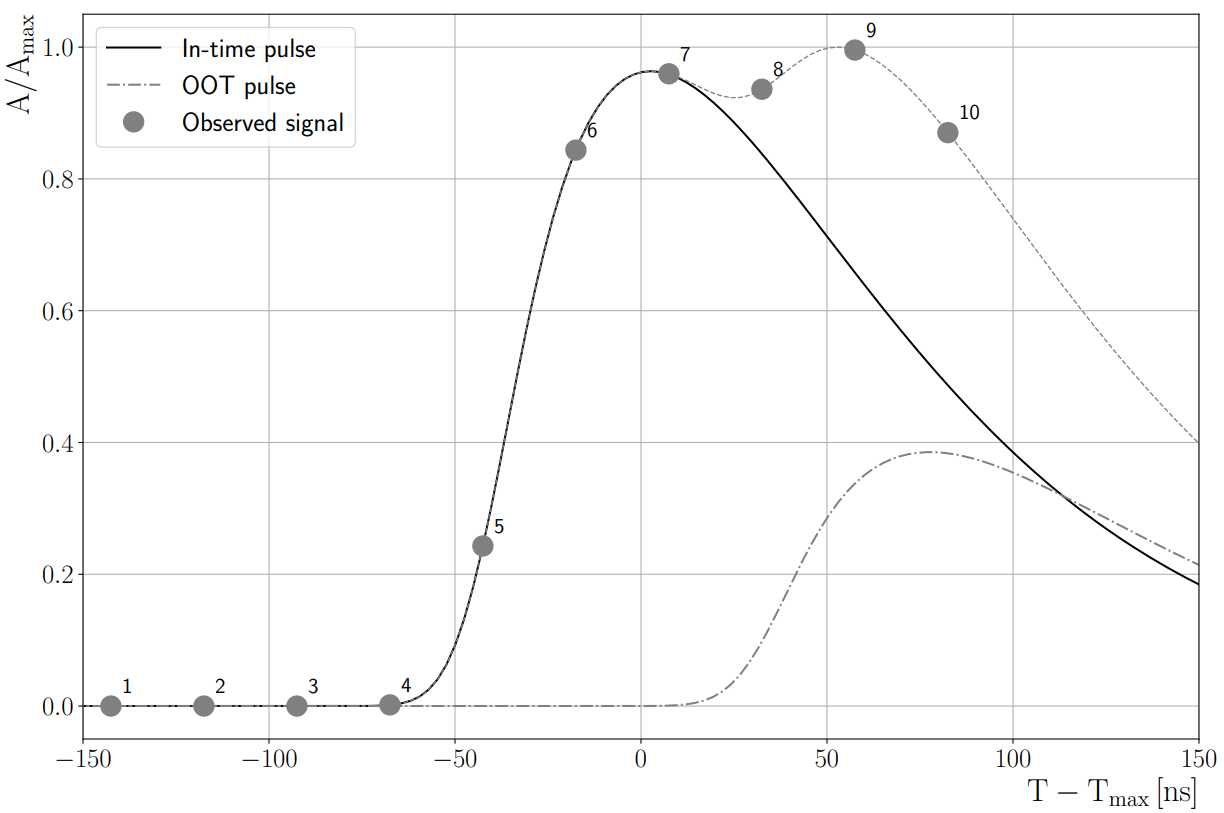
\includegraphics{fig/sec_reco/two_pulses.png}}
\caption{The fitted pulse for a simulated event with twenty average pileup events and 25 ns bunch spacing as a function of the difference between the time (T) of the ADC sample and the time (Tmax) of the maximum of the pulse and the amplitude of the pulse (A) normalized by the maximum amplitude of the pulse (A$_{max}$). The dots represent the 10 discrete samples of the measured pulse shape (dashed line) that is a superposition of an in-time pulse (solid line) and an OOT pulse (dashed line). 
%Note that the samples are numbered starting at 0 instead of 1. 
}
\label{tec_multifit2}
\end{center}
\end{figure}

The ECAL time reconstruction developed for Run 1 was utilized through the start of Run 3.  With this time reconstruction it was found that the fast time constants of PbWO$_{4}$ scintillation and the response of the readout electronics allows a time resolution on the order of 100's of picoseconds for isolated interactions \cite{Collaboration_2010}.  Residual channel-to-channel time offsets are corrected with appropriate constants derived from data. This timing information, combined with topological information of the energy deposits, is exploited at reconstruction level to reject signals inconsistent with the emission of scintillation light by particles produced in proton-proton collision events. These spurious signals include those arising from direct ionization in the APD sensitive region ( spikes ) as well as signals arising from beam halo muons, cosmic rays, electronic noise, detector material interactions, and OOT-PU. In Run 1 it was found that, for the conditions prevalent at that time, the residual contamination of these spurious deposits has a negligible impact on reconstruction \cite{CMS-NOTE-2010-012}. The signal arrival time for a rechit is reconstructed  by comparing the relative phase of the sample pulse amplitudes to the expected pulse shape. In originally developed algorithm used the ratios of consecutive amplitude samples to reconstruct the time.  This method did not take into account the challenges presented by the increasing PU present in Run 2 and Run 3 to the time reconstruction. The ratio method algorithm, and the challenges it faced, is discussed in Section~\ref{sec:algo1}. In order to account for these changes a new time reconstruction, the cross correlation method ( CC ), was developed during Run 2.  The CC time reconstruction will be  presented in Section~\ref{sec:algo2}.
 
